%% SECTION HEADER /////////////////////////////////////////////////////////////////////////////////////
\section{Temperature effect on the \acs{gw} propagation}
\label{sec:temp}
 
Since \ac{gw} measurements take place in the millisecond range, temperature changes in the inspected structure are negligible.
Therefore, \ac{gw} propagation can be modelled for the stationary temperature field.
It is assumed that the temperature field can be obtained from temperature sensors at the moment of \ac{gw} excitation.
A uniform temperature field was assumed in the model for simplicity.

In order to carry out the temperature-dependent \ac{sem} simulations, only changes in the elastic modulus of the \ac{hsc} components are considered.
The density changes are neglected. For the \ac{cfrp} skin, the modulus is calculated as per the methodology described in \cite{chamis1983simplified,salamone2009guided}.
The significant changes in mechanical properties under temperature occur mainly in the polymer matrix, while the variation in the carbon fibre properties has a negligible effect on wave propagation.
In this model \cite{salamone2009guided, hopkins2012extreme}, the reduction of Young’s modulus of the resin \(E_m\) with temperature variation is assumed as:
\begin{eqnarray}
	E_m(T)=F_m E_{m}(T_r),
	\label{eq:factor_temp}
\end{eqnarray}
where \(E_{m}(T_r)\) is the Young’s modulus of resin at the reference temperature and \(F_m\) is the temperature degradation factor as proposed in \cite{chamis1983simplified}:
\begin{eqnarray}
F_m=\sqrt{\frac{T_{g0}-T}{T_{g0}-T_r}},
\label{eq:em_temp}
\end{eqnarray}
where \(T_{g0}\) is the glass transition temperature and \(T_r\) is the reference temperature.
Eq. (\ref{eq:em_temp}) is also applicable to determine the elastic modulus of the adhesive layer bonding of the core to the skins, while for aluminium, the linear temperature dependence given by Hopkins et al. \cite{hopkins2012extreme} as:
\begin{eqnarray}
	E_a(T)=E_a(T_{r})+\num{4e7}(T_r-T).
	\label{eq:aluminium_temp}
\end{eqnarray}
The Young modulus and Poisson ratio of the sensors are in the form proposed by Lanza et al. \cite{lanza2008temperature}:
\begin{eqnarray}
	\left(E_{11}\right)_{pzt}(T) & = & \left[\left(E_{11}\right)^{-1}_{pzt}(T_r) + \num{2.142857e-14}(T_r-T)\right]^{-1},\\
	\left(E_{33}\right)_{pzt}(T) & = & \left[\left(E_{33}\right)^{-1}_{pzt}(T_r) + \num{0.777142e-14}(T_r-T)\right]^{-1},\\
	\nu_{pzt}(T) & = & \nu_{pzt}(T_r) + \num{13e-3}(T_r-T).
	\label{eq:pzt_temp}
\end{eqnarray}
The piezo- and electromechanical properties are taken into account based on the temperature characteristics provided by the manufacturer.
The characteristics are approximated by the linear functions in the analysed range, as it is shown in Fig.~\ref{fig:pzt_manuf}.
The approximation functions are given in the form:
\begin{eqnarray}
	\boldsymbol{\epsilon}(T) & = & \boldsymbol{\epsilon}_r - 3.292(T_r-T),\\
	\boldsymbol{d}(T) & = & \boldsymbol{d}_r - \num{1.742857}(T_r-T),\\
	\boldsymbol{e}(T) & = & \boldsymbol{d}(T)\,\boldsymbol{C}_{PZT}(T),
	\label{eq:piezo_temp}
\end{eqnarray}
were \(\boldsymbol{d}\) is the charge constant matrix, \(\boldsymbol{e}\) is the piezoelectric coupling coefficients matrix and \(\boldsymbol{C}_{PZT}\) is the elastic stiffness matrix.
The piezo constant matrices for reference temperature are provided by manufacturer as follows:
\begin{eqnarray}
	\boldsymbol{d} & = & \left[
	\begin{array}{cccccc}
	0 & 0 & 0 & 0 & 669 & 0\\
	0 & 0 & 0 & 669 & 0 & 0\\
	-208 & -208 & 443 & 0 & 0 & 0\\
	\end{array}\right] \times10^{-12}\ \unit[per-mode = symbol]{\coulomb\per\newton},\\
	\boldsymbol{\epsilon} & = & \left[
	\begin{array}{ccc}
	802 & 0 & 0\\
	0 & 802 & 0\\
	0 & 0 & 729\\
\end{array}\right] \times10^{-11}\ \unit[per-mode = symbol]{\farad\per\meter},
\end{eqnarray}

\begin{table}[H]
	\small
	\tabcolsep=0.5cm
	\centering
	\caption{\label{tab:properties}The mechanical properties of the materials at reference temperature of +20\unit{\degreeCelsius}.}
	\begin{tabular}{ccccc}\toprule
		\multirow{2}{*}{\textbf{Material}} & $\boldsymbol{E_{11}}$ & $\boldsymbol{E_{33}}$ & $\boldsymbol{\nu_{12}}$ & $\boldsymbol{\rho}$ \\ & \unit{\giga\pascal} & \unit{\giga\pascal} & -- & \unit[per-mode = symbol]{\kilogram\per\cubic\meter}\\
		\midrule
		Carbon & 275 & 27 & 0.2 & 1900\\
		Epoxy & 3.43 & 3.43 & 0.35 & 1250\\
		Aluminium & 69 & 69 & 0.33 & 2770\\
		Epoxy adhesive & 6 & 6 & 0.34 & 1200\\
		Cyanoacrylate glue & 3 & 3 & 0.34 & 1200\\	
		\ac{pzt} &  59 & 47 & 0.31 & 7850\\
		\bottomrule
	\end{tabular}
\end{table}

\begin{figure}
	\begin{center}
		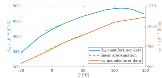
\includegraphics[width=0.95\textwidth]{Chapter_3/pzt_piezo_temp}
	\end{center}
	\caption{Temperature-dependent piezoelectric characteristics of the \acf{pzt} provided by the manufacturer, \textbf{(a)} relative change of the charge constant solid line and linear approximation dashed line, \textbf{(b)} relative change of the permittivity solid line and linear approximation dashed line.}
	\label{fig:pzt_manuf}
\end{figure}

The complete set of temperature-dependent coefficients required for the simulations are shown in Figs.~\ref{fig:isoEG}-\ref{fig:pztEEps}.
\begin{figure}
	\begin{center}
		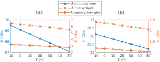
\includegraphics[width=0.95\textwidth]{Chapter_3/isoEG}
	\end{center}
	\caption{Temperature-dependent \textbf{(a)} Young's modulus (E) and \textbf{(b)} shear modulus (G) for isotropic materials used in the simulations.}
	\label{fig:isoEG}
\end{figure}
\begin{figure}
	\begin{center}
		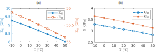
\includegraphics[width=0.95\textwidth]{Chapter_3/cfrpEG}
	\end{center}
	\caption{Temperature-dependent \textbf{(a)} Young's modulus (E\(_{11}\), E\(_{33}\)) and \textbf{(b)} shear modulus (G\(_{12}\), G\(_{23}\)) for the \acf{cfrp} skin}
	\label{fig:cfrpEG}
\end{figure}
\begin{figure}
	\begin{center}
		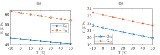
\includegraphics[width=0.95\textwidth]{Chapter_3/pztEG}
	\end{center}
	\caption{Temperature-dependent \textbf{(a)} Young's modulus (E\(_{11}\), E\(_{33}\)) and \textbf{(b)} shear modulus (G\(_{12}\), G\(_{23}\)) for the \acf{pzt}}
	\label{fig:pztEG}
\end{figure}
\begin{figure}
	\begin{center}
		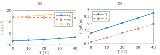
\includegraphics[width=0.95\textwidth]{Chapter_3/pztEEps}
	\end{center}
	\caption{Temperature-dependent \textbf{(a)} piezoelectric coupling coefficients (e\(_{31}\), e\(_{15}\), e\(_{33}\) and \textbf{(b)} electric permittivity (\(\epsilon_{11}\), \(\epsilon_{33}\)) for the \acf{pzt}}
	\label{fig:pztEEps}
\end{figure}


